\documentclass{abnt}
\usepackage[brazil]{babel}
\usepackage[utf8]{inputenc}
\usepackage[num]{abntcite}
\usepackage{graphicx}
\usepackage{url}
\usepackage{caption}
\usepackage{listings}

\lstset{
basicstyle=\small\sffamily,
numbers=left,
numberstyle=\tiny,
frame=tb,
columns=fullflexible,
showstringspaces=false
}

\graphicspath{{imagens/}}

\begin{document}
\autor{André Taiar Marinho Oliveira}

\titulo{A look into new programming languages}

\orientador[Orientador:\\]{Prof. Dr. Fernando Magno Quintão Pereira}

\comentario{Apresentado como de trabalho na disciplina de Atividades Práticas Integradoras do Curso de Bacharelado em Sistemas de Informação da UFMG}

\instituicao{Universidade Federal de Minas Gerais \par Instituto de Ciências
Exatas \par Departamento de Ciência da Computação}

\local{Belo Horizonte} \data{2015/2}

\capa
\folhaderosto

\begin{resumo}
There are hundred of programming languages out there. Which one should we use?
Which help do we have to choose well? How do they compare to each other? This
document is an attempt to provide some answers to these questions. Naturally, it
would not be possible to provide complete answers: as I mentioned, there are too
many programming languages. Nevertheless, we chose four languages with a
potential to grow in importance in the coming years. These programming languages
are Elixir, Rust, Dart, and Ceylon. During this project, we shall be
talking about each one of them. These discussions will be in breath, not in
depth. Their goal is to provide the reader with the minimum of information
necessary to compare them, and who knows, to lure one or other interested person
in learning them in a greater level of details. In any case, we hope to
contribute a bit to the popularization of these programming languages, which -
likely - will be paramount to the development of computer science in the next
ten years.\\


\textbf{Palavras-chaves}: saas, gestão, estratégia.
\end{resumo}

\sumario %comando que gera o sumário automaticamente
\renewcommand*\listfigurename{LISTA DE FIGURAS}
\listoffigures %comando que gera um sumário para a lista de figuras do texto automaticamente


\chapter{INTRODUÇÃO}

O planejamento estratégico das organizações surgiu em em meados da década de 60
se tratando de uma metodologia que permite estabelecer a direção a ser seguida
pela organização e visa um maior grau de interação com o ambiente aonde ela
atua. É um processo aonde se observa a organização por diversos ângulos,
direcionando os seus rumos e monitorando as suas ações de forma concreta.
Grandes empresas se beneficiam diretamente do planejamento através de gestão
estratégica de suas atividades, seja em um escopo amplo ou em projetos e sub
produtos dentro de sua cadeia de produção.

Micro e pequenas empresas não costumam se beneficiar diretamente do planejamento
estratégico e muitos motivos podem ser os motivos para que isso ocorra. O
assunto de Gestão Estratégica é bastante amplo; muitas técnicas podem ser
utilizadas e diversas análises podem ser feitas em cima de uma mesma organização
e dominar a utilização e entendimento destas ferramentas pode ser bastante
complicado para alguém não especialista na área. Mesmo que um gestor de
organização tenha domínio ou conhecimento específico sobre algumas destas
ferramentas do gerenciamento, utilizá-las parcialmente ou separadamente não é
tão efetivo quanto aplicá-las em uma sequência correta de passos com informações
integradas entre as etapas do processo. Além destes motivos, geralmente o gestor
de pequenas e médias empresas já tem grande parte do seu tempo tomado por
cumprir as funções do próprio metabolismo da organização, faltando tempo a ser
investido em conhecer melhor tais ferramentas e sua correta aplicação dentro do
cenário de sua organização.

A proposta desta monografia é desenvolver o protótipo de um sistema que agrupe
diversas ferramentas de gestão para planejamento estratégico de forma integrada.
A utilização destas ferramentas se dará de tal forma que o usuário do sistema
interaja com a plataforma seguindo um fluxo definido de atividades que se
integram e geram resultados mais relevantes em seu conjunto de especialidades.
Este fluxo de utilização deve ser o mais didático possível, permitindo que um
gestor de organização, independente de sua familiaridade com ferramentas de
gestão estratégica, consiga utilizar corretamente os conceitos e obter
informações para avaliação e direcionamento do negócio.

Espera-se que deste trabalho resulte um protótipo funcional que seja distribuído
como um Software as a Service (Saas)\cite{Turner2003}. A principal
característica em um software como serviço é a não aquisição das licenças mas
sim pagar pelo uso como um serviço. Funcionando em ambiente web, espera-se que
o modelo possibilite a aquisição do produto por um baixo preço, tornando sua
utilização viável para micro e pequenas empresas e atraindo mercado maior devido
a escala que pode alcançar.\\

\chapter{CONTEXTUALIZAÇÃO E TRABALHOS RELACIONADOS}

A temática deste trabalho é fortemente apoiada sob três pilares principais e
multidisciplinares. Primeiramente, será desenvolvido um sistema e isso será a
parte mais técnica do trabalho e reunirá conceitos de engenharia de software,
cloud computing e gerenciamento de projetos. Em segundo lugar, o software deve
implementar soluções para gerenciamento estratégico, abrangendo ferramentas
baseadas em teorias de gestão estratégica de organizações. Por fim, o sistema e
as informações devem ser disponibilizados por meio de uma interface intuitiva e
com forte apelo didático, apoiando o usuário às informações necessárias para
alimentar o sistema e, em alguns pontos críticos, instruindo o usuário na
operação que deve ser feita no sistema.

\section{Gestão estratégica}

% contextualização da gestão estratégica

O planejamento estratégico é considerado um instrumento administrativo
relacionado à estratégia empresarial, pois é a sustentação do desenvolvimento e
da implementação de estratégias empresariais\cite{OLIVEIRA1991}.

% descrição básica dos módulos selecionados
% explicar o gráfico e exemplificar um modelo de fluxo no sistema

\begin{figure}[!htb]
	\centering
	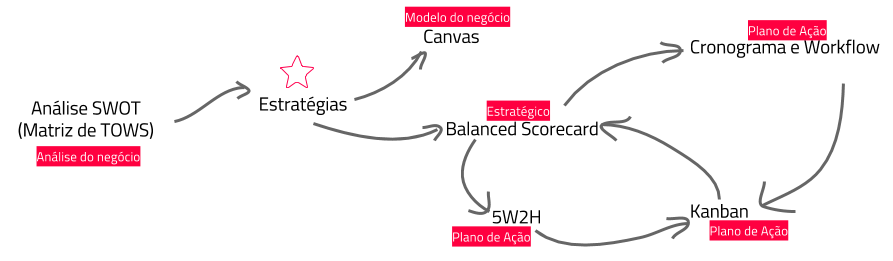
\includegraphics[width=\textwidth]{fluxograma_exemplo.pdf}
	\caption{Exemplo de fluxo de trabalho possível no sistema}
	\label{Rotulo}
\end{figure}

\section{Didática}

% validar a idéia de facilidade de uso do sistema com relação à usuários leigos
% adicionar ideias de interação e ajudo do sistema
% validar coisas através de IHC

\section{Software (as a Service)}

% contextualizar o software como serviço
% contextualizar as metodologias que serão utilizadas

\chapter{DESENVOLVIMENTO DO TRABALHO}

\section{Ceylon language}

\subsection{How did it appear?}

Red Hat\cite{1_1} is the world's leading provider of open source software
solutions and it has initiated and sponsored\cite{1_2} the development
of the Ceylon programming language. Ceylon is first and foremost an open source
community project.

According to the language's F.A.Q\cite{1_3}, Ceylon was designed to be a
modern Java with better specification, as we can see in the excerpt:

\begin{quote}
Well, we've been designing and building frameworks and libraries for Java for
ten years, and we know its limitations intimately. And we're frustrated. The
most recent releases of Java go some distance to alleviating some problems,
but even the newest language features strain to accommodate past mistakes and
the requirement for full backward compatibility.
But much of our frustration is not even with the Java language itself. The
extremely outdated class libraries that form the Java SE SDK are riddled with
problems. Developing a great SDK is a top priority of the project.
\end{quote}

\subsection{Why was it designed and implemented?}

Ceylon has a lot of interesting features but, we can start with this
definition on the homepage\cite{1_4}: \textit{"Ceylon is a language for writing
large programs in teams"}. The language is deeply influenced by Java and it was
designed and implemented by people who were hugely involved with Java. People
like Gavin King, the lead of the Ceylon project in Red Hat and also the creator
of Hibernate\cite{1_5} (the most popular Object Relational Mapper for Java) and
other projects in the Oracle's platform.

Modularity is in the very core of the Ceylon language. When a Ceylon's code is
compiled, it produces module archives. In fact is very similar to Java's
modules. It generates a *.car file, with *.class files zipped on it. Just
like Java's *.jar. You'll never be exposed to unpacked *.class files in
Ceylon. So here we got 2 conclusions. The first one is that the compiler
really forces the modularity and facilitates the distribution of the generated
code. The second one is that the Ceylon compiled code runs on the Java Virtual
Machine (JVM). This second fact is very important because by running on the JVM,
Ceylon's code is fully interoperable with Java, the Java SDK and its libraries.
In fact, this interoperability is a major priority of the project.

This is an example of the use of the Java's HashMap data structure on a Ceylon
program:

\begin{lstlisting}[label=cujhm,caption=Ceylon using Java HashMap]
import java.util { HashMap }

value javaHashMap = HashMap<String,Integer>();
javaHashMap.put("zero", 0);
javaHashMap.put("one", 1);
javaHashMap.put("two", 2);
print(javaHashMap.values());
\end{lstlisting}

Ceylon runs on the JavaScript virtual machine too. In fact the Ceylon's compiler
can generate JavaScript code if told to do so. It generates modular JavaScript
in the CommonJS modules format. We'll see more on JavaScript generation in the
future.

\begin{lstlisting}[label=cjs,caption=Ceylon JavaScript]
dynamic {
    dynamic req = XMLHttpRequest();
    req.onreadystatechange = void () {
        if (req.readyState==4) {
            document.getElementById("greeting")
                    .innerHTML = req.status==200
                            then req.responseText
                            else "error";
        }
    };
    req.open("GET", "/sayHello", true);
    req.send();
}
\end{lstlisting}

Ceylon's project always tells how important is the toolset for a complete and
successful programing project so it ships with a really great Integrated
Development Environment (IDE) built on a Eclipse plug-in. We'll see more
detailed information on the {install and run} section below.

\subsection{How can we use it, e.g., install and run?}

By running in the JVM, the Ceylon's compiler got the advantage to run
on every operating system which has a Java Virtual Machine implementation. It  
runs both on Java 7 and Java 8 (prior versions are not supported). So before
installing the Ceylon package, be sure to have the correct Java version
installed. On this work, I'm using the 1.1 version of the language, released on
09 October 2014.

For installation on a Mac, you can use the Homebrew installer:

\begin{verbatim}
$ brew update
$ brew install ceylon
\end{verbatim}

There are packages for both Debian and Fedora/Red Hat GNU/Linux flavors on the
project's download page\cite{1_10}.

For a platform agnostic installation, download the zip archive
(\url{http://ceylon-lang.org/download/dist/1_1_0}),
unzip on your system's prefered folder and add the \textbf{/ceylon-1.1.0/bin}
folder to the path of your system. In a unix-like system you can do that by
adding the line below on the \textbf{~/.bashrc} file of you user's directory:

\begin{verbatim}
$ export PATH="/path/to/ceylon-1.1.0/bin:$PATH"
\end{verbatim}

Now let's check if the installation works. By forcing the modularity, Ceylon
implies some conventions on the compilation process. At first the code we'll
write must be on a \textbf{"source"} directory. So place the following code on a
file called \textbf{"./source/hello.ceylon"}:

\begin{lstlisting}[label=hello,caption=Ceylon Hello World]
shared void hello() {
  print("Hello Ceylon!");
}
\end{lstlisting}

Outside the \textbf{source's} folder, run the command:

\begin{verbatim}
$ ceylon compile source/hello.ceylon
\end{verbatim}

Checkout the \textbf{module} folder created on the same level as the 
\textbf{source} folder. Check it's content for the \textit{*.car} file and some
others. To run the compiled source, run the following command:

\begin{verbatim}
$ ceylon run --run hello default
\end{verbatim}

\subsection{Simple programs}

I will demonstrate some features of the language by writing some simple programs
and analyzing some points right after it.

\subsubsection{The treelike structure, simple classes and visibility}

I'll use this example to illustrate the treelike structure that Ceylon has.
Ceylon's named argument lists provide an elegant way for initializing objects
and collections. The goal of this facility is to replace the use of XML for
expressing hierarchical structures such as documents, user interfaces,
configuration and serialized data.

I'll use this notation to create a binary search tree and make a depth-first
in-order traversal.

\begin{lstlisting}[label=ctls,caption=Ceylon treelike structure]
shared class Node(val, left = null, right = null) {
	shared Integer val;
	shared Node? left;
	shared Node? right;
}

shared void caminhamento_central(Node b) {
	if(exists next = b.left) {
		caminhamento_central(next);
	}
	process.write(b.val.string + " ");
	if(exists next = b.right) {
		caminhamento_central(next);
	}
}

shared void run() {
	Node arvore = Node {
		val = 1;
		left = Node {
			val = 2;
			left = Node {
				val = 4;
				left = Node { val = 8; };
				right = Node { val = 9; };
			};
			right = Node {
				val = 5;
				left = Node { val = 10; };
				right = Node { val = 11; };
			};
		};
		right = Node {
			val = 3;
			left = Node {
				val = 6;
				left = Node { val = 12; };
				right = Node { val = 13; };
			};
			right = Node {
				val = 7;
				left = Node { val = 17; };
				right = Node { val = 15; };
			};
		};
	};

	caminhamento_central(arvore);
	print("");
}
\end{lstlisting}

The result of this program must be:

\begin{verbatim}
8 4 9 2 10 5 11 1 12 6 13 3 17 7 15
\end{verbatim}


Look at the word \textit{shared} on some points of the example. This \textit{shared}
annotation marks a declaration as being visible outside the scope in which it is
defined, or a package as being visible outside the module to which it
belongs\cite{1_6}.

It's all about visibility\cite{1_7}. Classes, interfaces, functions, values,
aliases, and type parameters have names. Occurrence of a name in code implies a
hard dependency from the code in which the name occurs to the schema of the
named declaration. We say that a class, interface, value, function, alias, or
type parameter is visible to a certain program element if its name may occur in
the  code that belongs to that program element. The visibility of a declaration
depends upon where it occurs, and upon whether it is annotated \textit{shared}. 

\subsubsection{Random numbers and Java interoperability}

Ceylon's SDK is under constant development\cite{1_8} and there aren't a random
numbers implementation yet. But Ceylon can use the Java SDK, so I'll use the
Java random numbers interface to work on a Ceylon's simple example.

\begin{lstlisting}[label=w1,caption=Random number from Java]
// Import from Java SDK
import java.util { Random }

shared Integer getRandomInteger(Integer a, Integer b, Random r) {
	value range = b - a + 1;
	value fraction = (range * r.nextDouble());
	return (fraction + a).integer;
}

shared void run() {
    Random random = Random();
    for(number in 1..100) {
        print(getRandomInteger(1, 100, random));
    }
}
\end{lstlisting}

To use the Java SDK (and other libraries from outside the language's SDK) you
must use the module structure that is conventioned in the language. I'll use
this example to show it.

Save the code above on a file called \textbf{random.ceylon} inside of the
following structure of directories: \textbf{./source/example/random/}. This
structure corresponds to the namespace of the module we are creating. It's just
like Java always did.

Inside this same folder, create the file \textbf{module.ceylon}. It is the file
that will specify the dependencies our module have with external resources (like
Java libraries) and formalize it's namespace. The content of this file must be:

\begin{lstlisting}
module example.random "1.0.0" {
    import java.base "8";
}
\end{lstlisting}

The \textit{java.base} module in JDK has Java base packages such as
\textit{java.lang}, \textit{java.util}, \textit{java.io}, \textit{java.net},
\textit {java.text}, NIO and security\cite{1_9}. All done, inside of the
project's root, run the command:

\begin{verbatim}
$ ceylon compile
\end{verbatim}

The module will be compiled with the correct dependencies and the files will be
generated in the correspondent directory of the module (in our example, it
would be $./modules/example/random/1.0.0/$). Then we can run the code
with the command:

\begin{verbatim}
$ ceylon run example.random
\end{verbatim}

The program will execute calling the method \textit{run} (like the \textit{main}
method in Java) inside the package \textit{example.random}.

\section{Ceylon language usage}

To show some more interesting features of Ceylon, I wrote a version of the
Producer-consumer problem. This is a classic example of a multi-process
synchronization problem. It describes two processes, the producer and the
consumer, who share a common, fixed-size storage (buffer) used as a queue. The
producer's job is to generate a piece of data, put it into the storage and start
again. At the same time, the consumer is consuming the data (i.e., removing it
from the storage) one piece at a time. The problem is to make sure that the
producer won't try to add data into the storage if it's full and that the
consumer won't try to remove data from an empty storage\cite{2_1}.

The implementation relies strongly of the Java Thread libraries. The Producer
and the Consumer objects runs on different threads, each instance of each
object. The Storage class manage the additions of the producers and the
remotion of the consumers on the buffer. For synchronization I used the Java's
Semaphore class.

Let's see the code and I'll give the explanations:

\begin{lstlisting}[label=cpc,caption=Ceylon Producer-Consumer example]
import ceylon.collection { ArrayList }
import java.util.concurrent { Semaphore }
import java.lang { Thread, Math }

shared Integer getRandomInteger(Integer a, Integer b) {
	value range = b - a + 1;
	value fraction = (range * Math.random());
	return (fraction + a).integer;
}

class Producer(Storage storage, shared actual Integer id) extends Thread() {

	void produce() {
		if(Math.random() < 0.5) {
			storage.add(this);
		}
	}

	shared actual void run() {
		while(true) {
			this.produce();
			this.sleep(getRandomInteger(1, 4) * 1000);
		}
	}

}

class Consumer(Storage storage, shared actual Integer id) extends Thread() {

	void consume() {
		if(Math.random()  < 0.5) {
			storage.get(this);
		}
	}

	shared actual void run() {
		while(true) {
			this.consume();
			this.sleep(getRandomInteger(1, 4) * 1000);
		}
	}

}

class Storage(shared Integer storageSpaces) {

	value buffer = ArrayList<Integer>(storageSpaces);
	variable Integer lastEmpty = 0;
	value m = Semaphore(1);

	for(i in 0..(this.storageSpaces - 1)) {
		this.buffer.push(0);
	}

	shared void get(Producer|Consumer actor) {
		m.acquire();
		assert(actor is Consumer);
		print("[Consumer " + actor.id.string + "] Wants to consume!");
		if(this.lastEmpty == 0) {
			print("[Storage] I have nothing for you now. Look: ");
		} else {
			this.lastEmpty--;
			this.buffer.set(this.lastEmpty, 0);
			print("[Storage] Ok, I got a thing for you.");
		}
		m.release();
		this.printBuffer();
	}

	shared void add(Producer|Consumer actor) {
		m.acquire();
		assert(actor is Producer);
		print("[Producer " + actor.id.string + "] Produced something.");
		if(this.lastEmpty == this.storageSpaces) {
			print("[Storage] I'm full! Can't take it right now, look:");
		} else {
			this.buffer.set(this.lastEmpty, 1);
			this.lastEmpty++;
			print("[Storage] Tank you! I'll store it.");
		}
		m.release();
		this.printBuffer();
	}

	shared void printBuffer() {
		m.acquire();
		process.write("[ ");
		for (load in this.buffer) {
			process.write(load.string + " ");
		}
		print("]");
		m.release();
	}

}

shared void run() {
	value storage = Storage(15);

	value p1 = Producer(storage, 1);
	value p2 = Producer(storage, 2);

	value c1 = Consumer(storage, 1);
	value c2 = Consumer(storage, 2);

	p1.start();
	p2.start();

	c1.start();
	c2.start();
}
\end{lstlisting}

The first thing we see are the imports. We are already used to them, in the
first article where I used already some Java interoperability and explained the
concept of modules. Every of these things are used here.

\subsection{Toplevel functions}

After that, we can see a function called \textit{getRandomInteger}. In Ceylon, this is a
\textit{toplevel function}. A toplevel function declaration, or a function declaration
nested inside the body of a containing class or interface, may be annotated
\textit{shared} (in the last article, I talked about the shared annotation and the
visibility issues). A toplevel shared function is visible wherever the package
that contains it is visible.

Another interesting thing about \textit{toplevel} functions in Ceylon is that they can
be called by external programs on the system. On the example, I'll modify the
function a little so we can see what is going on:

\begin{lstlisting}[label=cri,caption=Ceylon random integer function]
shared Integer getRandomInteger(Integer a = 1, Integer b = 5) {
	value range = b - a + 1;
	value fraction = (range * Math.random());
	value gen = (fraction + a).integer;
	print(gen);
	return gen;
}
\end{lstlisting}


The toplevel function must have no parameters (or default value parameters) so
you can call her externally. By placing our program inside a module called
\textit{prodcons} (see the module session on the first article), we can compile
and run the program like:

\begin{verbatim}
$ ceylon compile
$ ceylon run --run prodcons::getRandomInteger prodcons
\end{verbatim}

The random integer numbers between $[1, 5[$ will be generated by the program and
printed on the screen.

\subsection{Classes}

We have then, the class \textit{Producer} which is the very same class of the
\textit{Consumer}, except it calls different methods of the \textit{Storage} class. The
first interesting thing we can see is that Ceylon 1.1 has no constructor
methods. Since the earliest versions of the language, it supports a streamlined
syntax for class initialization where the parameters of a class are listed right
after the class name, and initialization logic goes directly in the body of the
class\cite{2_2}.

We can instantiate the class Producer like this:

\begin{lstlisting}[label=cpc,caption=Ceylon Producer-Consumer example]
value prod = Producer(Storage(15), 1);
\end{lstlisting}

The ability to refer to parameters of the class directly from the members of the
class has the intuit to cut down on verbosity. However, there are moments when
we would really appreciate the ability to write a class with multiple
initialization paths, something like constructors in Java. The constructors are
being implemented on Ceylon and will be available in the next versions of the
language.

The annotation \textit{shared} on the parameter \textbf{id} says that this is like a Java's
\textit{public} member of the class. \textbf{storage} is not annotated, so it is like a
private one.

Look at the annotation \textit{actual} that is used in the same \textbf{id} parameter and in
the \textbf{run} method. It tells that, inside the inheritance tree of possible
values (since the two classes extends the Thread Java class) that could
overwrite the method or the variable, this is the very one that will do it. So,
\textbf{shared id} is overwriting the parameter id (probably on the Thread Java
class) and \textbf{shared run} is overwriting a run method (surely on the Thread Java
class). In the case of Interfaces, the word to tell that a class implements
(from Java) an interface is \textbf{satisfies}; so a class \textbf{satisfies} an
interface. The annotation \textbf{actual} is used to tell what method is
\textbf{satisfying} the Interface's specification.

\subsection{Collections, sequences and tuples}

Ceylon SDK has a great library that implements every kind of collections, just
like Java does. There are interfaces and classes to implement all sort of
operations involving \textit{ArrayList}, \textit{LinkedList}, 
\textit{PriorityQueue}, \textit{HashSet}, \textit{HashMap}, \textit{TreeSet},
\textit{TreeMap} etc\cite{2_3}. In our example, I used an \textit{ArrayList}
(which is the implementation of a list using arrays) to store the production of
the Producer.

In the example, I used a loop to initialize every cell of the \textit{buffer}
list with the value zero. In the for loop, I used a \textbf{Sequence} to
generate the iterable value. Sequence is a type that in the first time could
look very familiar to a Java array but in fact they are very different. First of
all, the sequence is a \textbf{immutable} type and not a mutable concrete type
like the array. We can't set the value of an element like:

\begin{lstlisting}[label=cpc,caption=Ceylon Producer-Consumer example]
String[] operators = .... ;
operators[0] = "^"; //compile error
\end{lstlisting}

This following code, doesn't compile too:

\begin{lstlisting}[label=cpc,caption=Ceylon Producer-Consumer example]
for (i in 0..operators.size-1) {
    String op = operators[i]; //compile error
    // ...
}
\end{lstlisting}

The index operation $operators[i]$ returns an optional type \textit{String?},
which cannot be assigned to the type \textit{String}. Instead, if we need access
to the index, we use the special form of \textbf{for}:

\begin{lstlisting}[label=cpc,caption=Ceylon Producer-Consumer example]
for (i -> op in operators.indexed) {
    // ...
}
\end{lstlisting}

Ceylon has the \textbf{tuple} type too. It might be a very common use for the
most of those who already worked with a language that has tuples.

\begin{lstlisting}[label=cpc,caption=Ceylon Producer-Consumer example]
[Float,Float,String] point = [0.0, 0.0, "origin"];
\end{lstlisting}

\subsection{Type system}

Every value in a Ceylon program is an instance of a type that can be expressed
within the Ceylon language as a class. The language does not define any
primitive or compound types that cannot, in principle, be expressed within the
language itself.

Each class declaration defines a type. However, not all types are classes. It is
often advantageous to write generic code that abstracts the concrete class of a
value. This technique is called polymorphism. Ceylon features two different
kinds of polymorphism:

\begin{enumerate}
	\item \textbf{subtype polymorphism}, where a subtype \textit{B} inherits a supertype \textit{A}, and 
	\item \textbf{parametric polymorphism}, where a type definition \textit{A<T>} is parameterized by a generic type parameter T.
\end{enumerate}

Ceylon, like Java and many other object-oriented languages, features a single
inheritance model for classes. A class may directly inherit at most one other
class, and all classes eventually inherit, directly or indirectly, the class
\textit{Anything} defined in the module \textit{ceylon.language}, which acts as the root of
the class hierarchy.

In our example, we use a parameter of the methods \textit{add} and  \textit{get} which is
\textit{Producer|Consumer} type. This type means that, whateaver a \textit{Producer} or a
\textit{Consumer} parameter passed the this method, it'll work. The methods doesn't
need this, I place'em there just for exemplification. In Ceylon, this is called
\textbf{Union types}. For any types \textit{X} and \textit{Y}, the union, or disjunction, \textit{X|Y}, of
the types may be formed. A union type is a supertype of both of the given types
\textit{X} and \textit{Y}, and an instance of either type is an instance of the union type.

\subsection{Assertions and exceptions}

The assert statement validates a given condition, throwing an
\textit{AssertionException} if the condition is not satisfied. A distinguishing
characteristic of Ceylon is that exceptions aren't used to represent programming
errors. The Ceylon creators thinks that exceptions like \textit{NullPointerException},
\textit{ClassCastException} and \textit{IndexOutOfBoundsException} should never occur in at
runtime in a production system. They represent problems that must be fixed by
the programmer editing code, tend to hide the \"corner\" condition they represent
from someone reading the code and are much too low-level to carry any useful
information about the real problem. Because of that, Ceylon tries to encode
these \"corner\" conditions into the type system.
The compiler won't let you write:

\begin{lstlisting}[label=cpc,caption=Ceylon Producer-Consumer example]
print(process.arguments[1].uppercased);
\end{lstlisting}

This code isn't well-typed because $process.arguments[1]$ is of type
\textit{String?}, reflecting the fact that there might not be a second element in the
$list process.arguments$. Instead you're forced to at least take into
account the possibility that there are less than two arguments:

\begin{lstlisting}[label=cpc,caption=Ceylon Producer-Consumer example]
if (exists arg = process.arguments[1]) {
    print(arg.uppercased);
}
else {
    throw Exception("missing second argument");
}
\end{lstlisting}

Obviously, the code is a little bigger than the initial code we had but of
course the problem is very much clear, semantic and the readers of the code
would understand the problem behind the size of the arguments in a much clearer
way.

\subsection{Concurrency}

In our example, inside of the methods \textit{get} and \textit{add} of the \textit{Storage} class is
where we would have concurrency problems\cite{2_1}. To solve this potential
problems, the class uses synchronization implemented with semaphores. I used the
Semaphore class from Java \textit{"acquiring"} and \textit{"releasing"} the
execution flow whatever some of the Threads are updating the \textit{buffer} or
printing in the screen.

In Java is very common to use the \textit{synchronized} method annotation to tell a
Thread that this method have race conditions, and the JVM takes care of the
concurrency. To use it with Ceylon, I had to specifically put the call to the
synchronization methods because it doesn't have the annotation nor any kind of
compatibility with it.

\chapter{CONCLUSÕES E TRABALHO FUTUROS}

O projeto de interação entre os módulos do sistema demonstrou-se com o tempo ser
extremamente mais oneroso do que o que foi estimado no início do projeto. Também
é visível que o plano inicial de desenvolver muitos módulos e ferramentas de
gestão seria inviável ao longo de um semestre letivo. Neste ponto, a metodologia
ágil que foi escolhida para gerenciamento do projeto ajudou a refinar as tarefas
que existiam no \textit{backlog} do projeto, priorizando o que provavelmente
daria mais visibilidade ao projeto e que poderia ser relevante no contexto de um
sistema de gestão estratégica: o módulo de \textit{Balanced Scorecard}.

% TODO: falta algum elemento intermediário

Um produto mínimo viável como o que foi idealizado nesse trabalho parece ter um
potencial de crescimento muito grande. Como visto, o fluxo do projeto idealizado
foi muito grande em relação ao o que consegui desenvolver ao longo de um
semestre letivo. Por se tratar de um projeto com um certo apelo comercial,
pretendo continuar desenvolvendo o produto e investir mais esforço na produção
de um sistema mais completo.

\bibliography{bibliog}

\end{document}
